\documentclass[hyperref={pdfpagelabels=false},usepdftitle=false]{beamer}
\usepackage{../templates/myStyle}

\begin{document}
\selectlanguage{english}

\title{\titleText}
\subtitle{Bachelor's thesis of Martin Thoma}
\author{\tutor}
\date{5th of June, 2014}
%\subject{Programmieren}

\frame{\titlepage}

\frame{
    \frametitle{Contents}
    \setcounter{tocdepth}{1}
    \tableofcontents
    \setcounter{tocdepth}{2}
}

%\AtBeginSection[]{
%    \InsertToC[sections={\thesection}]  % shows only subsubsections of one subsection
%}

\section{What is my Bachelor's thesis about?}
\subsection{Online and offline recognition}

\begin{frame}{What is my Bachelor's thesis about?}
    \begin{itemize}
        \item Recognition of handwritten mathematical symbols
        \item On-line recognition, not OCR!
        \item Given a series of points $(x(t), y(t), b(t))$\\
              I want to get the \LaTeX{} command.
    \end{itemize}
\end{frame}

\begin{frame}{Why did I work on this topic?}
    \begin{itemize}
        \item \LaTeX{} is easy as soon as you know the \textbackslash{}commands.
        \item It's hard to find the \LaTeX{} command of single symbols.
        \item It's much harder to find complete formulas.
    \end{itemize}

    For now: recognition of isolated symbols.
\end{frame}

\section{write-math.com}
\subsection{Write Math}

\begin{frame}{write-math.com}
    \begin{itemize}
        \item a website where users can add labeled training data and unlabeled
              data which they want to classify. I call this data \enquote{recording}
        \begin{figure}[ht]
            \centering
            \subfloat{
                \includegraphics[height=0.1\textwidth]{../images/279952.pdf}
            }%
            \qquad
            \subfloat{
                \includegraphics[height=0.1\textwidth]{../images/281507.pdf}
            }%
            \qquad
            \subfloat{
                \includegraphics[height=0.1\textwidth]{../images/287612.pdf}
            }%
            \qquad
            \subfloat{
                \includegraphics[height=0.1\textwidth]{../images/292175.pdf}
            }%
            \caption*{4 recordings}
        \end{figure}
        \item works with desktop computers and touch devices
        \item symbol recognition can be done by multiple classifiers
        \item users can contribute formulas as recordings and as \LaTeX{} answers
              for recordings
        \item users can vote for \LaTeX{} answers:
              \Large $\leq$, $\leqq$, $\leqslant$, \dots \normalsize
        \item user who entered the recording can accept one answer
    \end{itemize}
\end{frame}

\framedgraphic{Classify}{../images/classify.png}
\framedgraphic{Workflow}{../images/workflow.png}
% \framedgraphic{User page}{../images/user-page.png}
% \framedgraphic{Information about recordings}{../images/view.png}
% \framedgraphic{Symbol page}{../images/symbol.png}
% \framedgraphic{Training}{../images/train.png}
\framedgraphic{Ranking}{../images/ranking.png}


\begin{frame}[fragile]{Statistics}
    \begin{itemize}
        \item 127 users with at least 5 recordings
        \item $\num{1111}$ symbols, but only $\num{369}$ used for experiments
        \item $\num{235831}$ recordings (e.g. $\num{3489}$ times \verb+\int+, but only 50 times \verb+X+)
    \end{itemize}
\end{frame}

\begin{frame}{First classification worker}
    \begin{itemize}
        \item preprocessing: Scale to fit into unit square while keeping the aspect
              ratio
        \item applies greedy time warping
        \item compares a new recording with every recording
              in the database
        \item[$\Rightarrow$] Classification time is in $\mathcal{O}(\text{recordings})$,
              but we rather would like $\mathcal{O}(\text{symbols})$
        \item the current server / workflow can only handle about 4000 recordings
        \item[$\Rightarrow$] Another way to classify is necessary
    \end{itemize}
\end{frame}

\section{Preprocessing and Features}
\subsection{Preprocessing Algorithms}
\begin{frame}{Preprocessing Algorithms}
    \begin{columns}[T] % contents are top vertically aligned
    \begin{column}[T]{5cm} % each column can also be its own environment
        \begin{itemize}
            \item<1-> Normalizing
            \begin{itemize}
                \item<2-> Scaling
                \item<2-> Shifting
                \item<3-> Resampling
            \end{itemize}
            \item<1-> Noise reduction
            \begin{itemize}
                \item<4-> Smoothing (e.g. moving average)
                \item<5-> Dot reduction
                \item<6-> Filtering (by distance, speed or angle)
                \item<8-> Stroke connection
            \end{itemize}
        \end{itemize}
    \end{column}
    \begin{column}[T]{6cm} % alternative top-align that's better for graphics
        \only<2>{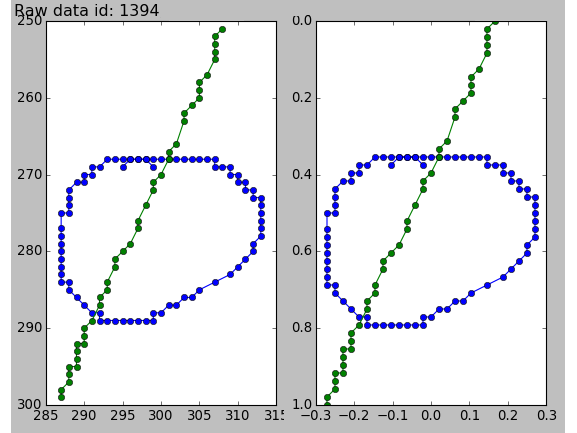
\includegraphics[width=6cm, keepaspectratio]{scale-and-shift.png}}
        \only<3>{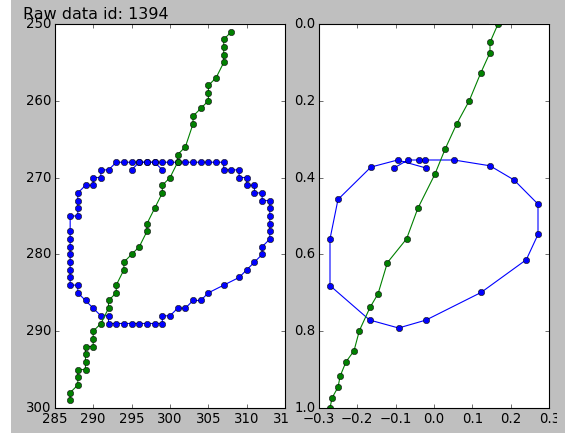
\includegraphics[width=6cm, keepaspectratio]{resampling.png}}
        \only<4>{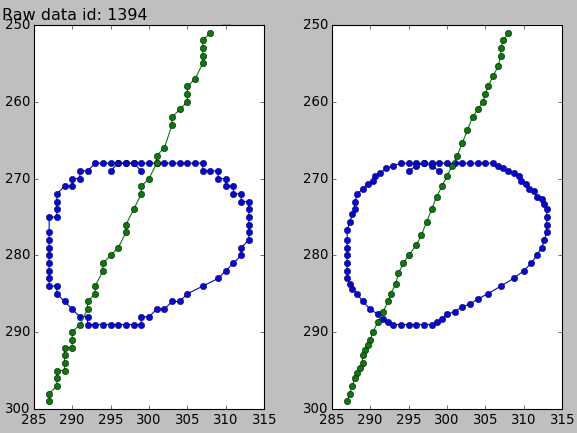
\includegraphics[width=6cm, keepaspectratio]{smooth-1-1-1.png}}
        \only<5>{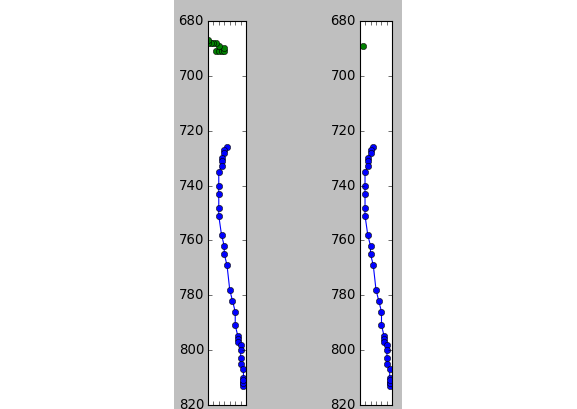
\includegraphics[width=6cm, keepaspectratio]{dot-reduction.png}}
        \only<6>{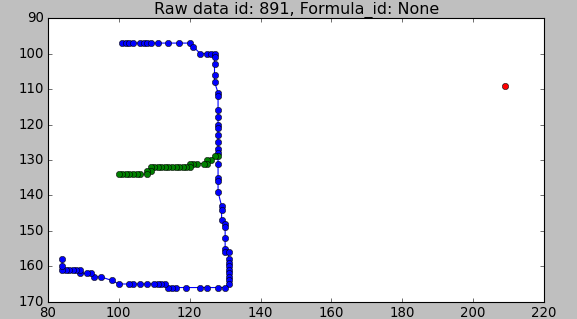
\includegraphics[width=6cm, keepaspectratio]{wildpoint-1.png}}
        \only<7>{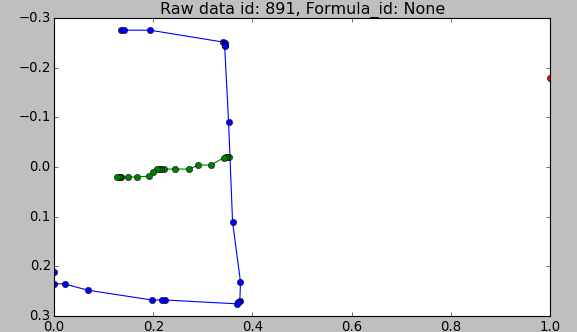
\includegraphics[width=6cm, keepaspectratio]{wildpoint-2.png}}
        \only<8>{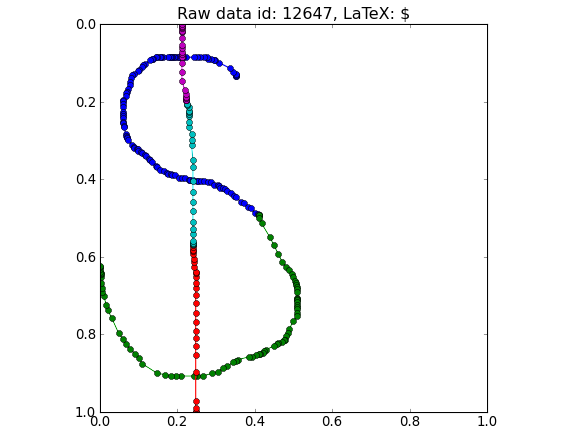
\includegraphics[width=6cm, keepaspectratio]{interrupted-stroke.png}}
    \end{column}
    \end{columns}
\end{frame}
\subsection{Features}
\begin{frame}{Features}
    \begin{columns}[T] % contents are top vertically aligned
    \begin{column}[T]{5cm} % each column can also be its own environment
        \textbf{Local Features}
        \begin{itemize}
            \item Coordinates
            \item Speed
            \item Binary pen pressure
            \item Direction
            \item Curvature
            \item Bitmap-environment
            \item Hat-Feature
        \end{itemize}
    \end{column}
    \begin{column}[T]{6cm} % alternative top-align that's better for graphics
        \textbf{Global Features}
        \begin{itemize}
            \item \# of dots ($i$, $j$, $\therefore$, $\because$, \dots)
            \item \# of strokes
            \item Center point coordinates
            \item Bitmap
            \item Bounding box (width, height, time)
            \item Re-curvature per stroke $s$ $\left ( \frac{\text{height}(s)}{\text{length}(s)} \right )$
            \item Ink
        \end{itemize}
    \end{column}
    \end{columns}
\end{frame}

\section{Neural Nets}
\subsection{Neural Net experiments}
\begin{frame}{Experiments}
    \textbf{Preprocessing:} Scaling, shifting and linear interpolation\\
    \textbf{Features:} Coordinates of 80 points (4 strokes with 20 points each)\\
    \textbf{Learning:} MLP, 300 epochs, LR of 0.1, Momentum 0.1

\begin{table}[h]
    \begin{tabular}{lrl}
    \toprule
    Topology                & Error    & Training time \\ \midrule
    160:500:369             & 30.62 \% & \hphantom{0}9min 08s      \\
    160:500:500:369         & 27.73 \% & 11min 49s     \\
    160:500:500:500:369     & 34.79 \% & 14min 09s     \\
    160:500:500:500:500:369 & 33.61 \% & 14min 06s     \\
    \bottomrule
    \end{tabular}
\end{table}

\end{frame}

\begin{frame}[fragile]{Examples of confusable symbols}
\begin{table}[ht]
    \centering
    \begin{tabular}{lc|lc}
        \textbf{\LaTeX}& \textbf{Rendered}   & \textbf{\LaTeX}& \textbf{Rendered} \\\midrule
        \verb+\sum+    & $\sum$         & \verb+$\Sigma$+        & $\Sigma$\\
        \verb+\coprod+ & $\coprod$      & \verb+$\amalg$+        & $\amalg$\\
        \verb+\perp+   & $\perp$        & \verb+$\bot$+          & $\bot$\\
        \verb+\models+ & $\models$      & \verb+$\vDash$+        & $\vDash$\\
        \verb+\emptyset+ & $\emptyset$  & \verb+$\diameter$+     & $\diameter$\\
        ~              & ~              & \verb+$\o$+            & $\o$\\
        ~              & ~              & \verb+$\varnothing$+   & $\varnothing$\\
        \verb+\Delta+  & $\Delta$       & \verb+$\triangle$+     & $\triangle$\\
        \verb+\varepsilon+ & $\varepsilon$ & \verb+$\mathcal{E}$+ & $\mathcal{E}$\\
    \end{tabular}
\end{table}

When those confusions are not counted as errors, the current best system
has an classification error rate of $12.7 \%$ (otherwise $22.2 \%$).

\end{frame}

\section{What will I do next?}
\subsection{What will I do next?}
\begin{frame}{What will I do next?}
    \begin{itemize}
        \item Include the currently best model in write-math.com
        \item Evaluate preprocessing steps
        \item Try other features
        \item Try other topologies / trainings (e.g. pretraining, newbob)
        \item Eventually try convolutional neural nets
    \end{itemize}
\end{frame}

% \subsection{Far future}
% \begin{frame}{What could be done?}
%     \begin{itemize}
%         \item Make use of audio data in a multimodal approach\\
%               e.g. $R$ and $\mathcal{R}$
%         \item Currently, the Lecture Translation system doesn't recognize math.\\
%               You get \enquote{integral of e raised to the power of x d x} instead
%               of $\int e^x \mathrm{d} x$.
%         \item Spoken math is ambigous: $\sqrt{a+b}$ vs. $\sqrt{a} + b$
%         \item The language model I create could help to find probable formulas
%         \item The platform could be used to get more input data of users
%     \end{itemize}
% \end{frame}

\section*{End}
\subsection{End}
\subsection{Image Sources}
\begin{frame}{Image Sources}
    \begin{itemize}
	\item \href{https://commons.wikimedia.org/wiki/File:PageRank-hi-res.png}{PageRank} by Felipe Micaroni Lalli
	\item screenshots of \href{http://www.dmoz.org}{www.dmoz.org}
	\item \href{https://commons.wikimedia.org/wiki/File:Hyperlink-Wikipedia.svg}{Hyperlink} by Bernard Ladenthin
	\item screenshots of \href{http://dontbubble.us}{dontbubble.us}
        \item \href{http://commons.wikimedia.org/wiki/File:Sergey_Brin.JPG}{Sergey Brin} by enlewof
        \item \href{http://commons.wikimedia.org/wiki/File:Larry_Page_laughs.jpg}{Larry Page} by aweigend
    \end{itemize}
\end{frame}

\framedgraphic{Thanks for Your Attention!}{../images/xi.png}

\end{document}
